\documentclass[border=15pt]{standalone}
\usepackage{tikz,amsmath,amssymb}
\usetikzlibrary{arrows.meta}
\usepackage{tikzcats}   % 原生保留 tikzcats

% ========== 配色方案 ==========
\definecolor{inFill}{RGB}{183,224,177}       % 浅绿 (H/2)
\definecolor{inLine}{RGB}{32,102,32}
\definecolor{blFill}{RGB}{190,225,245}       % 天蓝 (H/4)
\definecolor{blLine}{RGB}{40,110,170}
\definecolor{orFill}{RGB}{250,224,180}       % 橙黄 (H/8)
\definecolor{orLine}{RGB}{190,110,20}
\definecolor{yeFill}{RGB}{252,240,180}       % 鹅黄 (H/16)
\definecolor{yeLine}{RGB}{180,150,20}

\begin{document}
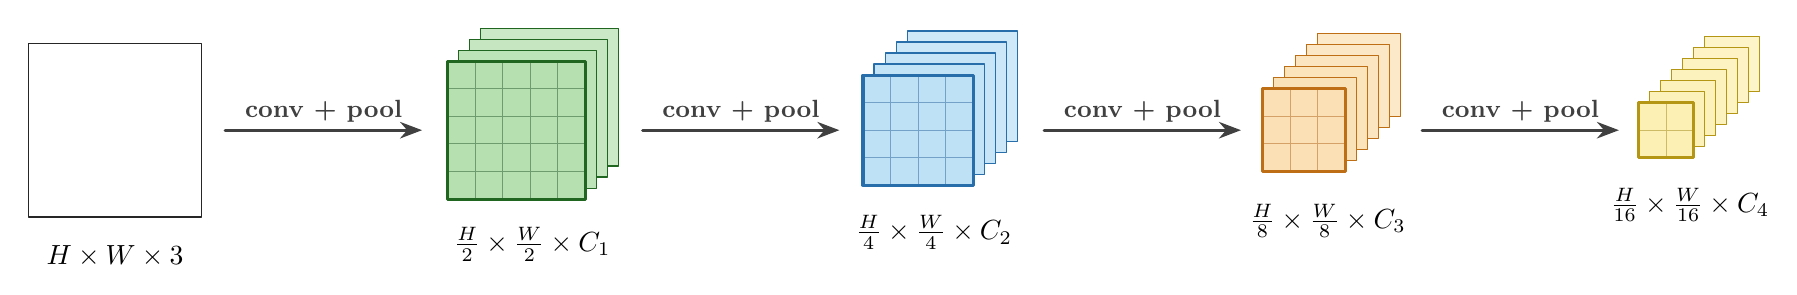
\begin{tikzpicture}[
    font=\normalsize, line join=round, line cap=round,
    every node/.style={inner sep=0pt, outer sep=0pt, align=center},
    arr/.style={->, >=Stealth, line width=1.1pt, darkgray}
  ]

  % ========== 宏：优化后的 3D 堆叠特征图 ==========
  \newcommand{\fstack}[6]{%
    \pgfmathsetmacro{\sz}{#4*#5}
    \pgfmathsetmacro{\half}{\sz/2}
    \foreach \k in {#3,...,1}{%
      \pgfmathtruncatemacro{\op}{round(100 - (28 * \k / #3))}
      \fill[#6Fill!\op, draw=#6Line, line width=.4pt]
        ({#1 - \half + 0.14*\k}, {#2 - \half + 0.14*\k}) rectangle ++({\sz}, {\sz});
    }
    \fill[#6Fill] ({#1 - \half}, {#2 - \half}) rectangle ++({\sz}, {\sz});
    \draw[step=#5, #6Line!65, line width=.35pt, shift={({#1 - \half}, {#2 - \half})}] (0,0) grid ({\sz}, {\sz});
    \draw[#6Line, line width=1.1pt] ({#1 - \half}, {#2 - \half}) rectangle ++({\sz}, {\sz});
  }

  % 输入猫咪图片 (2.2 x 2.2 cm)
  \newcommand{\catimg}[2]{%
    \draw[black!85, line width=.5pt, fill=white] ({#1-1.1},{#2-1.1}) rectangle ++(2.2,2.2);
    \node at (#1, #2) {\scalebox{0.185}{\tikz{\cat}}};
  }

  % 1. Input Image
  \catimg{1.1}{2.2}
  \node[font=\normalsize, text=black] at (1.1, 0.6) {$H\times W\times 3$};

  % 2. 阶段 1: H/2 (箭头长 2.5cm)
  \draw[arr] (2.5, 2.2) -- (5.0, 2.2) node[midway, above=3pt, font={\small\bfseries}] {conv + pool};
  \fstack{6.2}{2.2}{3}{5}{0.35}{in}
  \node[font=\normalsize, text=black] at (6.4, 0.75) {$\frac{H}{2}\times\frac{W}{2}\times C_1$};

  % 3. 阶段 2: H/4 (箭头长 2.5cm)
  \draw[arr] (7.8, 2.2) -- (10.3, 2.2) node[midway, above=3pt, font={\small\bfseries}] {conv + pool};
  \fstack{11.3}{2.2}{4}{4}{0.35}{bl}
  \node[font=\normalsize, text=black] at (11.5, 0.9) {$\frac{H}{4}\times\frac{W}{4}\times C_2$};

  % 4. 阶段 3: H/8 (箭头长 2.5cm)
  \draw[arr] (12.9, 2.2) -- (15.4, 2.2) node[midway, above=3pt, font={\small\bfseries}] {conv + pool};
  \fstack{16.2}{2.2}{5}{3}{0.35}{or}
  \node[font=\normalsize, text=black] at (16.5, 1.05) {$\frac{H}{8}\times\frac{W}{8}\times C_3$};

  % 5. 阶段 4: H/16 (箭头长 2.5cm)
  \draw[arr] (17.7, 2.2) -- (20.2, 2.2) node[midway, above=3pt, font={\small\bfseries}] {conv + pool};
  \fstack{20.8}{2.2}{6}{2}{0.35}{ye}
  \node[font=\normalsize, text=black] at (21.1, 1.25) {$\frac{H}{16}\times\frac{W}{16}\times C_4$};

\end{tikzpicture}
\end{document}